
\chapter{アンカーの発話区間検出精度}
\begin{figure}[H]
  \begin{center}
    \includegraphics[scale=0.5]{./figure/prob1_08.eps}
  \end{center}
  \caption{手法1によるアンカーの発話区間検出精度 ($Th_{time}=0.8$)}
\end{figure}

\begin{figure}[H]
  \begin{center}
    \includegraphics[scale=0.5]{./figure/prob1_09.eps}
  \end{center}
  \caption{手法1によるアンカーの発話区間検出精度 ($Th_{time}=0.9$)}
\end{figure}

\begin{figure}[H]
  \begin{center}
    \includegraphics[scale=0.5]{./figure/prob1_10.eps}
  \end{center}
  \caption{手法1によるアンカーの発話区間検出精度 ($Th_{time}=1.0$)}
\end{figure}

\begin{figure}[H]
  \begin{center}
    \includegraphics[scale=0.5]{./figure/prob1_11.eps}
  \end{center}
  \caption{手法1によるアンカーの発話区間検出精度 ($Th_{time}=1.1$)}
\end{figure}

\begin{figure}[H]
  \begin{center}
    \includegraphics[scale=0.5]{./figure/prob1_13.eps}
  \end{center}
  \caption{手法1によるアンカーの発話区間検出精度 ($Th_{time}=1.3$)}
\end{figure}

\begin{figure}[H]
  \begin{center}
    \includegraphics[scale=0.5]{./figure/prob1_14.eps}
  \end{center}
  \caption{手法1によるアンカーの発話区間検出精度 ($Th_{time}=1.4$)}
\end{figure}

\begin{figure}[H]
  \begin{center}
    \includegraphics[scale=0.5]{./figure/prob1_15.eps}
  \end{center}
  \caption{手法1によるアンカーの発話区間検出精度 ($Th_{time}=1.5$)}
\end{figure}

\begin{figure}[H]
  \begin{center}
    \includegraphics[scale=0.5]{./figure/prob3_08.eps}
  \end{center}
  \caption{手法3によるアンカーの発話区間検出精度 ($Th_{time}=0.8$)}
\end{figure}

\begin{figure}[H]
  \begin{center}
    \includegraphics[scale=0.5]{./figure/prob3_09.eps}
  \end{center}
  \caption{手法3によるアンカーの発話区間検出精度 ($Th_{time}=0.9$)}
\end{figure}

\begin{figure}[H]
  \begin{center}
    \includegraphics[scale=0.5]{./figure/prob3_10.eps}
  \end{center}
  \caption{手法3によるアンカーの発話区間検出精度 ($Th_{time}=1.0$)}
\end{figure}

\begin{figure}[H]
  \begin{center}
    \includegraphics[scale=0.5]{./figure/prob3_11.eps}
  \end{center}
  \caption{手法3によるアンカーの発話区間検出精度 ($Th_{time}=1.1$)}
\end{figure}

\begin{figure}[H]
  \begin{center}
    \includegraphics[scale=0.5]{./figure/prob3_12.eps}
  \end{center}
  \caption{手法3によるアンカーの発話区間検出精度 ($Th_{time}=1.3$)}
\end{figure}

\begin{figure}[H]
  \begin{center}
    \includegraphics[scale=0.5]{./figure/prob3_14.eps}
  \end{center}
  \caption{手法3によるアンカーの発話区間検出精度 ($Th_{time}=1.4$)}
\end{figure}

\begin{figure}[H]
  \begin{center}
    \includegraphics[scale=0.5]{./figure/prob3_15.eps}
  \end{center}
  \caption{手法3によるアンカーの発話区間検出精度 ($Th_{time}=1.5$)}
\end{figure}
